\section{Space complexity}
\label{sec:space}

We show that the expected salt length of the BHF matches the
information-theoretic lower bound on space complexity to leading order, for
both Bernoulli sets and Bernoulli maps, under both fixed predicate forms.
This is the familiar seed-index scale of seed-search
constructions~\cite{esposito2020recsplit,lehmann2024shockhash,lehmann2025seeds};
no novelty is claimed for it.

\subsection{General proof (maps)}

The BHF representation is the tuple $(h_k, b)$ or $(N, t, b)$.
The dominant term is the length of the salt $b$, which the algorithm discovers
by exhaustive search in order of increasing length.

\begin{theorem}[Success probability per trial]
\label{thm:success_prob}
The probability that a candidate salt $b$ yields a valid BHF for a map with
$m$ keys, false positive rate $\fprate$, and mean value encoding length $\mu$
is:
\begin{enumerate}[(i)]
    \item Equality predicate: $p_{\mathrm{eq}} = \fprate^{m-1} / 2^{m\mu}$.
    \item Threshold predicate: $p_{\mathrm{th}} = \fprate^{m} / 2^{m\mu}$.
\end{enumerate}
\end{theorem}
\begin{proof}
See \cref{thm:success_eq,thm:success_thresh}.
\end{proof}

\begin{theorem}[Space complexity of the BHF]
\label{thm:space}
The expected bit length of the BHF asymptotically achieves
\begin{equation}
    -\log_2 \fprate + \mu \;\; \si{bits \per element}
\end{equation}
as $m \to \infty$, for both predicate forms.
\end{theorem}
\begin{proof}
The algorithm searches through candidate salts in order of increasing bit
length.
By \cref{def:mapping}, the \nth candidate maps uniquely to a bit string.
The search terminates at the first success, which follows a geometric
distribution with parameter $p$ (where $p = p_{\mathrm{eq}}$ or
$p = p_{\mathrm{th}}$).

Let $\RV{Q} \sim \geodist(p)$ be the trial at which the first success occurs.
The salt bit length is $\RV{L} = \lfloor \log_2 \RV{Q} \rfloor$.

We bound $\Expect{\RV{L}}$ using the exact formula from
\cref{thm:expected_size}:
\begin{equation}
    \Expect{\RV{L}} = \sum_{n=1}^{\infty} q^{2^n - 1}
    = q + q^3 + q^7 + q^{15} + \cdots\,,
\end{equation}
where $q = 1 - p$.
To extract the leading-order behavior, note that
$\lfloor \log_2 x \rfloor \leq \log_2 x$ for all $x \geq 1$, so
\begin{equation}
    \Expect{\RV{L}} \leq \Expect{\log_2 \RV{Q}}
    \leq \log_2 \Expect{\RV{Q}} = -\log_2 p\,,
\end{equation}
where the second inequality is Jensen's (since $\log_2$ is concave).
For the lower bound, $\lfloor \log_2 x \rfloor \geq \log_2 x - 1$, so
\begin{equation}
    \Expect{\RV{L}} \geq \Expect{\log_2 \RV{Q}} - 1\,.
\end{equation}
Since $\RV{Q} \sim \geodist(p)$, $\Prob{\RV{Q} \leq a} \leq a p$ for all
$a \geq 0$.
Writing $\ell = -\log_2 p$,
\begin{equation}
    \Expect{(\ell - \log_2 \RV{Q})_{+}}
    = \int_0^\infty \Prob{\RV{Q} < 2^{\ell - u}}\, du
    \leq \int_0^\infty 2^{-u}\, du = \log_2 e\,,
\end{equation}
so $\Expect{\log_2 \RV{Q}} \geq -\log_2 p - \log_2 e$.
Together with the Jensen bound,
\begin{equation}
    -\log_2 p - \log_2 e - 1 \;\leq\; \Expect{\RV{L}} \;\leq\; -\log_2 p\,,
\end{equation}
so $\Expect{\RV{L}} = -\log_2 p + \mathcal{O}(1)$.
(An earlier version printed the closed form
$\Expect{\log_2 \RV{Q}} = -\log_2 p - (\log_2 e)(1 - p)\ln(1 - p)/p$; that
expression is the entropy of $\RV{Q}$ in bits, not its log moment.
At $p = 1/2$ it gives $2$, whereas $\Expect{\log_2 \RV{Q}} \approx 0.7326$ and
$\Expect{\lfloor \log_2 \RV{Q} \rfloor} \approx 0.6328$.)

\paragraph{Equality predicate.}
With $p = \fprate^{m-1}/2^{m\mu}$:
\begin{equation}
    \Expect{\RV{L}}
        = -(m-1)\log_2 \fprate + m\mu + \mathcal{O}(1)\,.
\end{equation}
Dividing by $m$ and taking $m \to \infty$:
\begin{equation}
    \frac{\Expect{\RV{L}}}{m} \to -\log_2 \fprate + \mu\,.
\end{equation}

\paragraph{Threshold predicate.}
With $p = \fprate^{m}/2^{m\mu}$:
\begin{equation}
    \Expect{\RV{L}}
        = -m\log_2 \fprate + m\mu + \mathcal{O}(1)\,.
\end{equation}
Dividing by $m$ and taking $m \to \infty$:
\begin{equation}
    \frac{\Expect{\RV{L}}}{m} \to -\log_2 \fprate + \mu\,.
\end{equation}
In both cases, the expected bits per element converges to the information-theoretic lower bound $-\log_2 \fprate + \mu$.
\end{proof}

\subsection{Set as corollary}

\begin{corollary}[Space complexity for sets]
\label{cor:set_space}
For a Bernoulli set ($\mu = 0$), the BHF achieves $-\log_2 \fprate$ bits per
element asymptotically.
\end{corollary}
\begin{proof}
Set $\mu = 0$ in \cref{thm:space}.
\end{proof}

\subsection{Finite-sample correction}

For finite $m$, the exact bits per element are:
\begin{equation}
    \frac{\Expect{\RV{L}}}{m} =
    \begin{cases}
        -\dfrac{m-1}{m}\log_2 \fprate + \mu + \mathcal{O}(1/m)
            & \text{(equality)}\,,\\[8pt]
        -\log_2 \fprate + \mu + \mathcal{O}(1/m)
            & \text{(threshold)}\,.
    \end{cases}
\end{equation}
The equality predicate is slightly more space-efficient for small $m$
(by $\log_2 \fprate / m$ bits per element) due to the adaptive $h_0$.

\subsection{Effect of false negatives}
\label{sec:fn_effect}

When $\fnrate > 0$, only $r = \lceil (1-\fnrate)m \rceil$ elements need to be
accepted.
For sets under the threshold predicate, a salt succeeds when at least $r$ of
the $m$ independent residues fall in the acceptance set, so the success
probability is the binomial tail
\begin{equation}
    s \;=\; \Prob{\bindist(m, \fprate) \geq r} \;\geq\; \fprate^{r}\,,
\end{equation}
where the inequality keeps only the event that a fixed $r$-subset is
accepted.
(An earlier version gave the probability $\fprate^{r-1}/2^{r\mu}$ that one
fixed subset succeeds under the equality predicate, which ignores the choice of
subset.)
The expected salt length is $-\log_2 s + \mathcal{O}(1)$, so the space per
element of the \emph{original} set is at most
\begin{equation}
    \frac{r}{m}\left(-\log_2 \fprate\right) + \mathcal{O}(1/m)
    \;\approx\; (1 - \fnrate)\left(-\log_2 \fprate\right)\,.
\end{equation}
This matches the lower bound in \cref{post:set_lb} to leading order in
$\log_2(1/\fprate)$; the bound itself holds only up to $\mathcal{O}(1)$ bits
per element~\cite[Prop.~1]{pagh2001lossy}.
For maps, each accepted key must also match its value bits, which adds
about $\mu$ bits per accepted key.

\subsection{Space complexity of the adaptive threshold}
\label{sec:adaptive_space}

The adaptive threshold stores the pair $(N, t)$ with no salt.
This yields a much lower per-element cost, but it does not meet the same
accuracy contract: the FPR is a random variable, and the recall is about
$p/m$ (\cref{sec:adaptive_contract}).

\begin{theorem}[Space complexity---adaptive threshold]
\label{thm:adaptive_space}
For a Bernoulli set ($\mu = 0$) with $m$ keys and modulus $N$, the adaptive
threshold BHF stores $(N, t)$ using
\begin{equation}
\label{eq:adaptive_bits}
    \lceil \log_2 N \rceil + \lceil \log_2 N \rceil
    \;=\; 2\lceil \log_2 N \rceil \;\;\si{bits}
\end{equation}
total (or $\lceil \log_2 N \rceil + \lceil \log_2(t+1) \rceil$ if $t$ is
encoded in fewer bits).
The per-element cost is
\begin{equation}
\label{eq:adaptive_per_element}
    \frac{2\lceil \log_2 N \rceil}{m} \;=\; \mathcal{O}\!\left(\frac{\log N}{m}\right) \;\to\; 0
    \quad\text{as } m \to \infty\,.
\end{equation}
\end{theorem}
\begin{proof}
The modulus $N$ requires $\lceil \log_2 N \rceil$ bits to encode, and the
threshold $t \in \{0,\ldots,N-1\}$ requires at most $\lceil \log_2 N \rceil$
bits.
There is no salt to store (for sets, $b = \epsilon$).
The per-element cost is the total divided by $m$, which vanishes as
$m \to \infty$ for any fixed $N$.
\end{proof}

\begin{remark}[Why the small per-element cost does not violate the lower bound]
\label{rem:lb_not_violated}
A random per-build FPR does not by itself escape the lower bound.
For each fixed non-member $x$, the probability that the adaptive structure
accepts $x$ is $\Expect{(T+1)/N}$, the expectation of the conditional FPR, and
the standard formulation of approximate membership already allows a randomly
constructed structure with this per-query guarantee~\cite{pagh2005}.
The reason the cost is small is that the adaptive structure answers a much
weaker question: its recall is about $p/m$, and its mean FPR is at least
$p/(m+1)$ (\cref{sec:adaptive_contract}).
With $\fnrate = 1 - p/m$ and $\fprate \approx p/(m+1)$, the lower bound of
\cref{post:set_lb} is $(p/m)\log_2(1/\fprate) - \mathcal{O}(1)$ bits per
element, which is vacuous in this regime: a data-independent coin achieves
recall equal to its FPR with no storage at all.
(Earlier versions attributed the gap to the randomness of the FPR alone and
called it the price of FPR certainty; that comparison held the recall
requirements unequal and is withdrawn.)
\end{remark}

\subsection{Comparison at the same accuracy contract}
\label{sec:price_certainty}

Earlier versions of this paper stated a ``price of FPR certainty'' theorem:
that the gap $m \log_2(1/\fprate^*)$ between the fixed-threshold and
adaptive-threshold encodings is the cost of committing to a fixed FPR rather
than of encoding membership.
That comparison held a fixed-threshold structure with recall $1$ against an
adaptive structure whose recall is about $p/m$, and it is withdrawn.
When both the recall and the FPR cap are held fixed, the adaptive rule
reduces to fixed-threshold search.

\begin{theorem}[Same-contract reduction]
\label{thm:price_certainty}
Let $\Set{S}$ be a set of $m$ elements ($\mu = 0$), fix a false positive cap
$\fprate^* = (t^*\!+1)/N$, and require at least $r$ accepted members.
For a candidate salt $b$, the adaptive event $\{\OS{r}{m} \leq t^*\}$ equals
the fixed-threshold event that at least $r$ residues are at most $t^*$.
Under the random oracle assumption its probability is
\begin{equation}
\label{eq:same_contract}
    s \;=\; \Prob{\bindist(m, \fprate^*) \geq r}\,,
\end{equation}
so the expected number of trials is $1/s$, a budget of $B$ independent salts
succeeds with probability $1 - (1-s)^B$, and the expected salt length is
$-\log_2 s + \mathcal{O}(1)$ bits.
At zero false negatives ($r = m$), $s = (\fprate^*)^m$ and the salt length
is $m \log_2(1/\fprate^*) + \mathcal{O}(1)$, as in \cref{thm:space}.
\end{theorem}

\begin{proof}
The $r$-th smallest residue is at most $t^*$ if and only if at least $r$
residues are at most $t^*$, which is the acceptance count of the fixed
threshold $t^*$.
Each residue is at most $t^*$ independently with probability $\fprate^*$,
giving \cref{eq:same_contract}.
Distinct salts are independent trials, which gives the trial count and the
budget formula; the salt length follows from \cref{thm:space}.
\end{proof}

For example, $m = 4$, $r = 3$, $\fprate^* = 1/5$ gives $s = 17/625$ by exact
enumeration, an expected $625/17$ trials, and success within eight trials
with probability about $0.198$.
This is ordinary binomial-tail search over a random codebook, the
single-seed mechanism analyzed in~\cite[Sec.~1.1]{lehmann2025seeds}; no new
construction follows from it.

\begin{remark}[Entropy of the salt index]
\label{rem:info_interp}
The salt is the index of the first success in a $\geodist(s)$ search.
Its entropy is
\begin{equation}
    \Entropy(\RV{Q})
    = -\log_2 s - \frac{(1-s)\log_2(1-s)}{s}
    = -\log_2 s + \mathcal{O}(1)\,,
\end{equation}
which equals $2$ bits at $s = 1/2$.
(An earlier version printed this formula with the wrong sign on the second
term, which gives $0$ at $s = 1/2$.)
The leading term is the standard seed-index scale.
\end{remark}

\Cref{fig:space_comparison} compares the per-element space cost of the two
fixed predicates.

\begin{figure}[ht]
\centering
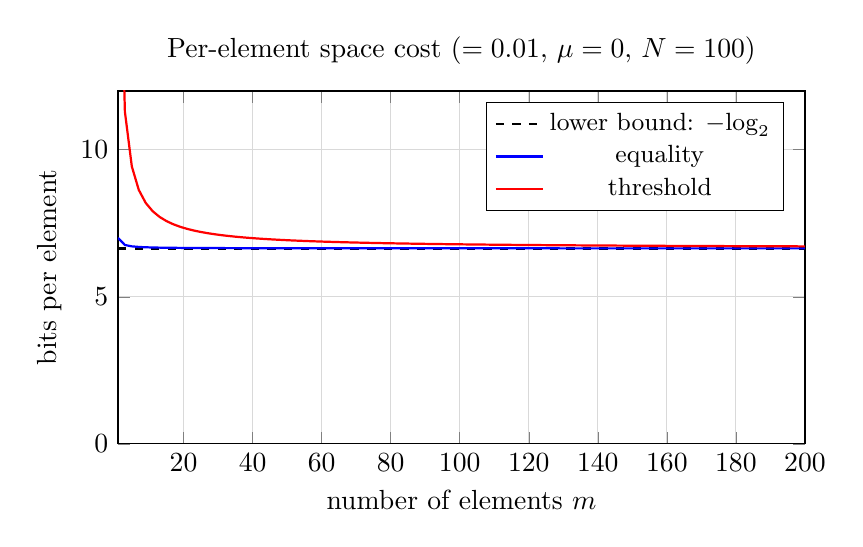
\begin{tikzpicture}
\begin{axis}[
    width=0.85\textwidth,
    height=0.5\textwidth,
    xlabel={number of elements $m$},
    ylabel={bits per element},
    xmin=1, xmax=200,
    ymin=0, ymax=12,
    legend style={at={(0.97,0.97)}, anchor=north east, font=\small},
    grid=major,
    grid style={gray!30},
    every axis plot/.append style={thick},
    title={Per-element space cost ($\fprate = 0.01$, $\mu = 0$, $N = 100$)}
]

% Lower bound: -log2(0.01) = 6.644
\addplot[black, dashed, domain=1:200, samples=100] {6.644};
\addlegendentry{lower bound: $-\!\log_2 \fprate$}

% Equality: -(m-1)/m * log2(eps) + O(1/m) ≈ (m-1)/m * 6.644 + log2(1/eps)/m
% success prob = eps^(m-1), salt bits ≈ (m-1)*log2(1/eps), plus k = log2(1/eps)
% total/m = (m-1)/m * 6.644 + 6.644/m = 6.644
% But for small m, the k bits overhead matters: (k + salt)/m
% k = ceil(log2(1/eps)) = 7 for eps=0.01
% salt ≈ (m-1)*6.644 bits
% total = 7 + (m-1)*6.644, per-element = 7/m + (m-1)/m*6.644
\addplot[blue, domain=1:200, samples=100] {7/x + (x-1)/x * 6.644};
\addlegendentry{equality}

% Threshold: salt ≈ m*6.644, plus ceil(log2 N) + ceil(log2 N) overhead
% total = 14 + m*6.644, per-element = 14/m + 6.644
\addplot[red, domain=1:200, samples=100] {14/x + 6.644};
\addlegendentry{threshold}

\end{axis}
\end{tikzpicture}
\caption{Per-element space cost for the equality and threshold BHF
    predicates with target $\fprate = 0.01$ ($N = 100$), from the leading
    terms of the analysis.
    Both converge to the information-theoretic lower bound
    $-\log_2\fprate \approx 6.64$ bits per element.
    The adaptive threshold is omitted: it does not meet the same recall
    requirement (\cref{sec:adaptive_contract}).}
\label{fig:space_comparison}
\end{figure}
